\documentclass[11pt]{article}

% Make margins smaller
\usepackage[top=0.65in, bottom=0.65in, left=0.6in, right=0.6in]{geometry}
% more advanced mathematical symbols
\usepackage{amsfonts}
\usepackage{amssymb}
\usepackage{amsmath}
\usepackage{bm}
\usepackage{bold-extra} % bold texttt
\usepackage{graphicx}
\usepackage{enumerate}
\usepackage[font=small,labelfont=bf]{caption} % Required for specifying captions to tables and figures
\usepackage{pgfgantt} % gantt chart!
\usepackage{titling}
\usepackage{setspace}
\renewcommand{\baselinestretch}{1.2} 

\graphicspath{ {./images/} }

% so that we can skip any number of items in an enumeration
\makeatletter
\newcommand{\skipitems}[1]{%
  \addtocounter{\@enumctr}{#1}%
}
\makeatother

\begin{document}

\title{\textbf{Virtual Reality Summative}}
\date{for 15th March 2019}
\author{Bradley Mackey}
\maketitle


\section*{Question Remarks}

\begin{enumerate}
\item 
\texttt{get\_raw\_imu\_data()} returns the raw data readings from the \texttt{.csv} file (given that it is located in the same directory), returning a 2D array of data rows.\\
\texttt{sanitize\_imu\_data(data)} cleans the data as specified, returning a 2D array of rows of the modified data.\\
\texttt{euler\_to\_qtrn(euler)} computes a quaternion $(a,b,c,d)$ from a given array of Euler angles $(x,y,z)$.\\
\texttt{qtrn\_to\_euler(qtrn)} computes the Euler angles $(x,y,z)$ for a given quaternion representation $(a,b,c,d)$.\\
\texttt{qtrn\_conj(qtrn)} takes a quaternion $(a,b,c,d)$ and returns its conjugate, $(a,-b,-c,-d)$.\\
\texttt{qtrn\_mult(qtrn\_1, qtrn\_2)} computes the product of 2 quaternions, returning this product $(a,b,c,d)$.

% NO REPORT REQUIRED FOR QUESTION #2
\skipitems{1} 

% QUESTION 3: Try a few different alpha values (e.g., 0.01, 0.1, ...), investigate and comment on their effect on drift compensation in your report (7 marks)

\item For the smallest values of $\alpha$ ($<0.001$), very little drift correction is applied and the headset is able to maintain smooth, albeit slightly misaligned motion after around 


\item Try a few different alpha values (e.g., 0.01, 0.1, ...), investigate and comment on their effect on drift compensation in your report (5 marks).
\end{enumerate}

\section*{Visualisations}

\begin{figure}[htp]

\centering
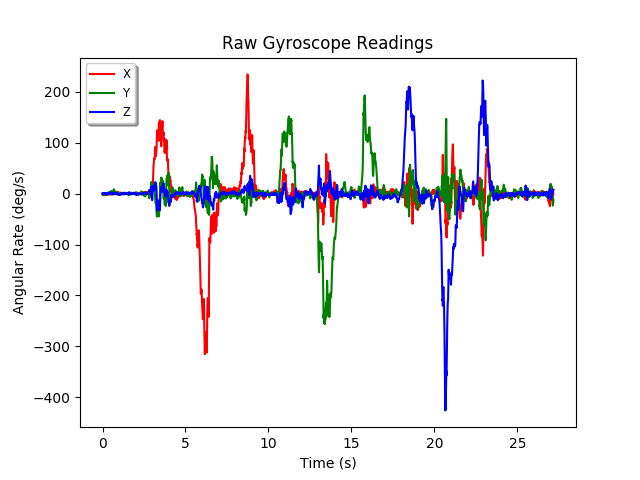
\includegraphics[width=.32\textwidth]{gyro-unaltered}\hfill
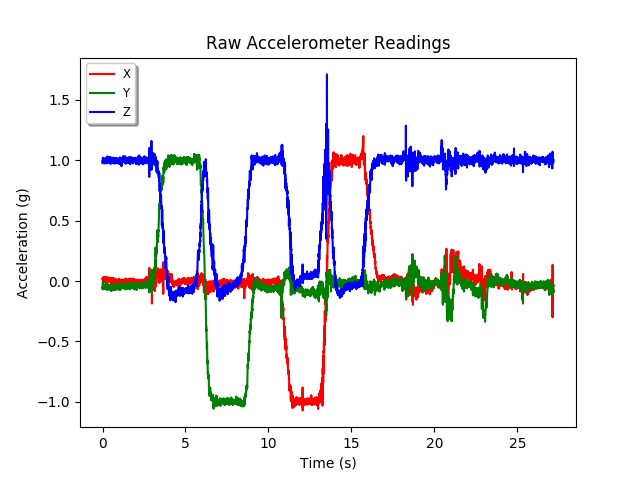
\includegraphics[width=.32\textwidth]{acc-unaltered}\hfill
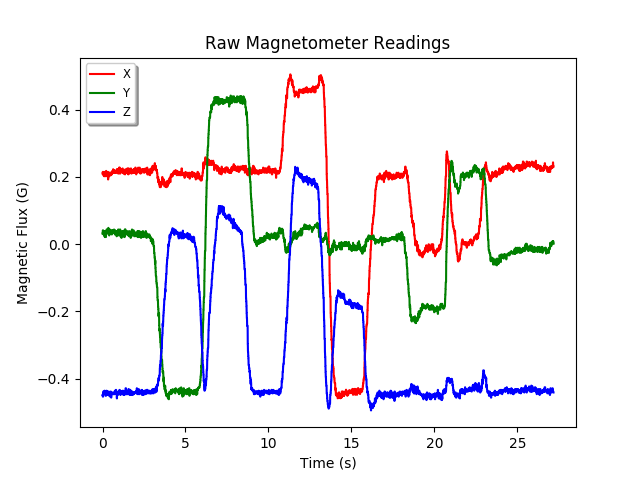
\includegraphics[width=.32\textwidth]{mag-unaltered}

\caption{Raw sensor readings from the IMU.}
\label{fig:figure3}

\end{figure}



\end{document}